% Claudia Porto, COMPLETE

The Perfect Matching Problem is a fundamental concept in graph theory, concerned with finding a matching in a graph where every vertex is paired with exactly one other vertex. In a perfect matching, no vertex is left unmatched, and all vertices are connected by edges in the matching. The Perfect Matching Problem is closely related to the Maximum Matching Problem, where the objective is to find the largest matching in a graph. The distinction between these problems lies in the requirement that a perfect matching must cover every vertex, while a maximum matching focuses on maximizing the number of edges in the matching, regardless of whether all vertices are matched. 

\subsection{Tutte's Theorem and the Perfect Matching Problem}

A key theoretical result in this domain is \textbf{Tutte’s Theorem}, which provides a necessary condition for the existence of a perfect matching in a graph. Tutte’s condition links the structure of a graph to its matching properties, serving as a critical tool in understanding and proving properties of perfect matchings. \cite{tutte1947some}

\subsubsection*{Preliminaries}

Consider an undirected graph \( G = (V, E) \). A matching is called a \emph{perfect matching} if it covers all the vertices of \( G \). The number of edges in a matching is called the \emph{size} of the matching. Note that a perfect matching has size \( n/2 \). Perfect matchings cannot exist in a graph with an odd number of vertices.

Given a graph \( G \) and a matching \( M \), an augmenting path \( P \) can be used to obtain a larger matching. By removing the even edges of \( P \) from \( M \) and adding the odd edges of \( P \) to \( M \), the size of the matching increases to \( |M| + 1 \). For a more detailed discussion of augmenting paths, see Chapter 2.

For a graph \( G = (V, E) \) and a vertex \( v \in V \), \( G - v \) is the graph \( G[V \setminus \{v\}] \). Similarly, for an edge \( e = (u, v) \) such that \( u, v \in V \) but \( uv \notin E \), \( G + e \) denotes the graph \( (V, E \cup \{e\}) \). Let \( q(G) \) denote the number of \textbf{odd components} in \( G \), where an odd component is a connected subgraph of G containing an odd number of vertices. 

\subsubsection*{Tutte's Condition for the Existence of a Perfect Matching}

\textbf{Tutte’s Theorem} provides the following condition for the existence of a perfect matching in a graph \( G \).

\begin{theorem}[Tutte's Theorem]
    An undirected graph \( G \) has a perfect matching if and only if, for every subset \( S \subseteq V \),
    \[
    |S| \geq q(G - S).
    \]
\end{theorem}

Let \( G \) have a perfect matching. Consider any subset \( S \), and let \( C \) be any odd component in \( G - S \). If we find a maximal matching in \( C \), exactly one vertex will remain unmatched (since \( |V(C)| \) is odd), which needs to be matched with a vertex in \( S \). Since this is true for every odd component, \( S \) needs to have enough vertices to match each odd component, i.e., \( |S| \geq q(G - S) \).
Any graph satisfying Tutte’s condition will contain a perfect matching. In the next section, we explore a proof of the sufficiency of Tutte’s condition.

\subsubsection*{Proof (Sketch) of Tutte’s Theorem}

To prove Tutte's condition, we show the contrapositive: 

Assuming \( G \) has no perfect matching, we find a subset \( S \subseteq V \) such that \( |S| < q(G - S) \), called a \textbf{bad set}. If \( |V| \) is odd, the empty set \( \emptyset \) is a bad set for \( G \). For \( |V| \) even, finding a bad set in \( G \) involves analyzing the following:

\begin{enumerate}
    \item \textbf{Edge-maximal graph \( G^* \):} Construct \( G^* \) by adding edges to \( G \) until adding any additional edge creates a perfect matching. Any bad set in \( G^* \) is also a bad set in \( G \).

    \item \textbf{Structure of bad sets:} A bad set in \( G^* \) has the following properties:
    \begin{enumerate}
        \item \( S \) is fully connected.
        \item Every vertex of \( S \) connects to every other vertex in \( G^* \).
        \item Each component of \( G^* - S \) is fully connected.
    \end{enumerate}
    These properties characterize all bad sets.

    \item \textbf{Finding a bad set in \( G^* \):} Group all universal vertices (those connected to every other vertex in \( G^* \)) into \( S \). This set \( S \) is a bad set if \( |S| < q(G^* - S) \).
\end{enumerate}

\subsubsection{Example of a Perfect Matching}

Consider a bipartite graph \( G = (V, E) \), where \( V = \{u_1, u_2, u_3, v_1, v_2, v_3\} \). The graph is partitioned into two sets: \[ U = \{u_1, u_2, u_3\},\quad V = \{v_1, v_2, v_3\} \]
A possible perfect matching for this graph is \( M = \{(u_1, v_1), (u_2, v_2), (u_3, v_3)\} \), which shows that each vertex in \( U \) is matched with exactly one vertex in \( V \), and vice versa. This perfect matching is illustrated in Figure \ref{fig:bipartite_graph}, where the matched edges are highlighted in red.

\begin{figure}[ht]
\centering
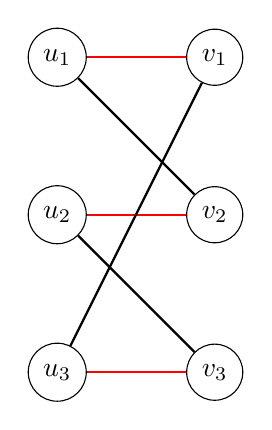
\begin{tikzpicture}[scale=1, transform shape]
    % Nodes for bipartite graph
    \node[draw, circle] (v1) at (2,2) {$v_1$};
    \node[draw, circle] (v2) at (2,0) {$v_2$};
    \node[draw, circle] (v3) at (2,-2) {$v_3$};
    \node[draw, circle] (u1) at (0,2) {$u_1$};
    \node[draw, circle] (u2) at (0,0) {$u_2$};
    \node[draw, circle] (u3) at (0,-2) {$u_3$};
    
    % Edges
    \draw[red, thick] (u1) -- (v1);   % Matching edge
    \draw[red, thick] (u2) -- (v2);   % Matching edge
    \draw[red, thick] (u3) -- (v3);   % Matching edge
    \draw[black, thick] (u1) -- (v2); % Non-matching edge
    \draw[black, thick] (u2) -- (v3); % Non-matching edge
    \draw[black, thick] (u3) -- (v1); % Non-matching edge
\end{tikzpicture}
\caption{A bipartite graph with perfect matching highlighted in red.}
\label{fig:bipartite_graph}
\end{figure}

\subsection{Reduction from Maximum Matching to Perfect Matching}

An interesting aspect of the Maximum Matching Problem in bipartite graphs is its relationship with the Perfect Matching Problem. A perfect matching in a bipartite graph is a matching where every vertex in both partitions is matched with exactly one vertex from the other partition. The key observation is that by constructing a bipartite graph that guarantees a perfect matching, solving the Perfect Matching Problem in this graph directly provides a solution to the Maximum Matching Problem \cite{cormen2009introduction}.

\subsubsection{Key Idea in Reduction}

The reduction from the Maximum Matching Problem to the Perfect Matching Problem for bipartite graphs involves constructing a new bipartite graph $G' = (V'_1 \cup V'_2, E')$ from the original bipartite graph $G = (V_1 \cup V_2, E)$. The construction ensures that $G'$ has a perfect matching, and solving the Perfect Matching Problem in $G'$ directly yields the maximum matching in $G$.

\begin{enumerate}
    \item \textbf{Graph Transformation:} 
    If the bipartite graph $G = (V_1 \cup V_2, E)$ does not already have a perfect matching, we add \textbf{dummy vertices} and edges to construct $G'$ such that $|V'_1| = |V'_2|$ and every vertex in $G'$ can be matched. Specifically:
    \begin{itemize}
        \item Add dummy vertices to the smaller partition (either $V_1$ or $V_2$) until both partitions have the same size.
        \item Add edges between the dummy vertices and all vertices in the opposite partition to ensure that $G'$ is still bipartite.
    \end{itemize}
    The resulting bipartite graph $G'$ is guaranteed to satisfy the conditions for a perfect matching. 
    \item \textbf{Finding the Maximum Matching:} Once $G'$ is constructed, we apply any algorithm for the Perfect Matching Problem to $G'$. Since $G'$ has a perfect matching, the solution provides a way to recover the maximum matching in $G$ by excluding any edges that involve dummy vertices.
\end{enumerate}

\subsubsection{Tutte's Matrix Method for Perfect Matching}

One notable algorithmic approach to solving the Perfect Matching Problem is the use of \textbf{Tutte's Matrix}, which gives an algebraic framework to determine and construct perfect matchings.\cite{yadav2023advanced, Geelen2000}

\subsubsection*{Construction of the Tutte Matrix:}

Given a bipartite graph $G = (V_1 \cup V_2, E)$, we construct a \textbf{skew-symmetric matrix} $M$ of size $n \times n$, where $n = |V_1| + |V_2|$, defined as:
\[
M_{ij} = 
\begin{cases} 
x_{ij} & \text{if } (v_i, v_j) \in E, \\
0 & \text{otherwise}.
\end{cases}
\]
Here, $x_{ij}$ are \textbf{indeterminates} for each edge $(v_i, v_j)$. 

\paragraph{Skew-Symmetric Matrix:} A \textbf{skew-symmetric matrix} is a square matrix $M$ that satisfies the condition:
\[
M_{ij} = -M_{ji} \quad \text{for all} \quad i, j.
\]
This means that the elements of the matrix are symmetric across the diagonal but with opposite signs. For example, if $M_{12} = 3$, then $M_{21} = -3$. Also, the diagonal elements of a skew-symmetric matrix are always zero.

In the case of the Tutte matrix, the off-diagonal elements correspond to the edges in the bipartite graph, and the diagonal elements are set to zero.

\subsubsection*{Determinant and Perfect Matching:}
For bipartite graphs, $M$ simplifies into a block structure. The determinant of $M$ is non-zero if and only if there exists a perfect matching in the graph. This property allows us to verify the existence of a perfect matching by symbolic determinant computation. Randomized methods or algebraic techniques can efficiently extract the perfect matching using the structure of $M$.

\subsubsection*{Reduction Context:}
In the context of this reduction, the construction of $G'$ ensures that $G'$ satisfies the necessary conditions for the Tutte Matrix method to succeed. Once $G'$ is transformed, the method confirms the existence of a perfect matching and facilitates its construction. If there exists a perfect matching, then there is a maximum matching.

\subsubsection{Complexity of the Reduction}

For bipartite graphs, the transformation involves adding at most $O(n)$ dummy vertices and edges, where $n = \max(|V_1|, |V_2|)$. If the Perfect Matching Problem can be solved in $T(n)$ time for bipartite graphs, the overall complexity of solving the Maximum Matching Problem via this reduction remains $O(T(n))$. For example, using algebraic methods like Tutte’s Matrix, the reduction is computationally efficient \cite{cormen2009introduction}.

\subsubsection{Implications of the Reduction}

This reduction has several significant implications for bipartite graphs:
\begin{itemize}
    \item \textbf{Efficiency:} By constructing a bipartite graph that guarantees a perfect matching, we simplify the Maximum Matching Problem while using well-studied algorithms for the Perfect Matching Problem.
    \item \textbf{Simplicity of Construction:} The use of dummy vertices and edges is straightforward in bipartite graphs, as they maintain the graph's partition structure and properties.
    \item \textbf{Algebraic Validation:} Tutte’s Matrix provides an algebraic method to confirm and construct perfect matchings.
\end{itemize}

For bipartite graphs, the Maximum Matching Problem can be effectively reduced to the Perfect Matching Problem by constructing a new graph $G'$ that guarantees a perfect matching. Using Tutte's theorem and matrix, this reduction ensures that solving the Perfect Matching Problem in $G'$ provides a direct solution to the Maximum Matching Problem in $G$.\cite{cormen2009introduction, berman1996algorithms, tutte1947some, Geelen2000}.